\htwo{Node.js}
\label{sec:nodejs}
\sectionauthor{Mersed Kečo}
Node.js ist eine plattformübergreifende Javascript-Laufzeitumgebung, die auf der V8 JS-Engine von Google basiert. Node.js wurde entwickelt um skalierbare Netzwerkanwendungen zu erstellen. Node.js wird von Ruby's "Event Machine" und Pythons "Twisted" beeinflusst und ähnelt diesen im Design. Die aktuelle Node.js-Version, die Version 17, während die Veröffentlichung der Version 18 für den 25. Oktober 2022 geplant ist.\cite{NodeInfo}

Laut "W3Techs" wird Node.Js von 1,2\% aller Webseiten genutzt. Auf das ganze Internet gerechnet sind das über 20 Millionen Webseiten, die mithilfe von Node.js betrieben werden. \cite{NodeInfo}\cite{Node}

\hfour{Architektur von Node.js}
Die von Node.js verwendete Architektur der "Single Threaded Event Loop" wird dazu verwendet, mehrere Clients gleichzeitig handzuhaben. Damit Endnutzer den  Unterschieden zwischen dieser und anderen Runtimes auf die Spuren kommen, ist es von oberster Priorität zu verstehen, wie "Multithreaded Concurrent Clients" in Java gehandhabt werden. \cite{NodeJs.dev}


Das Modell des "Multithreaded Request/Response" versendet Anfragen an verschiedene Clients, worauf der Server jede einzelne verarbeitet, bevor dieser darauf eine Antwort versendet. Jedoch ist es unvorteilhaft, dass mehrere Threads verwendet werden, um gleichzeitige Aufrufe zu verarbeiten. Verwendete Threads sind in einem Thread-Pool definiert und werden einkommenden Anfragen zugewiesen, um diese zu bearbeiten. \cite{Arocom}



\begin{figure}[H]
    \centering
    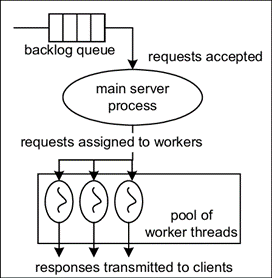
\includegraphics{media/NodeJs/MultiThreadedRequestResponse.png}
    \caption{Multithreaded Request/Response \cite{Multithreaded}}
\end{figure}

Thread-basierte Netzwerke sind ineffizient und äußerst schwierig zu verwenden. Node.js-Benutzer müssen sich wenige Sorgen machen, dass ein Prozess blockiert wird, da es keine Sperren gibt. Es gibt kaum Möglichkeiten, einen Prozess zu sperren außer wenn die Eingabe/Ausgabe mit synchronen Methoden der Node.js-Standardbibliothek durchgeführt wird. Aufgrund des "not locking" Mechanismus sind skalierbare Systeme mit Node.js sehr einfach zu entwickeln. 
Node.js arbeitet mit dem Modell der "Event Loop", welches natürlich seine eigenen Vor- und Nachteile mitbringt und diese mit dem folgenden Beispiel schrittweise erläutert werden.


\begin{figure}[H]
    \centering
    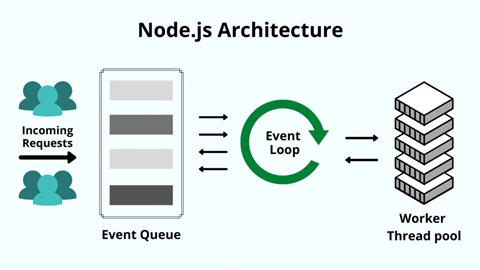
\includegraphics{media/NodeJs/NodeJsArchitektur.png}
    \caption{Node.Js Architektur \cite{ArchitekturFoto}}
\end{figure}


Node.js erlaubt nur eine begrenzte Anzahl an Threads in dem Threadpool, welche Anfragen bearbeiten. \cite{NodeJsArch}\cite{NodeJsArch2}

Sobald Anfragen reinkommen, werden diese von Node.js in eine Warteschlange namens "Event Queue" eingeordnet. \cite{NodeJsArch}\cite{NodeJsArch2}

Die Kernkomponente der Architektur kommt an diesem Punkt zum Einsatz, nämlich die Single Threaded "Event Loop". Dieser Thread wartet auf unbestimmte Zeit auf eingehende Anfragen. \cite{NodeJsArch}\cite{NodeJsArch2}

Bei einer eingehenden Anfrage holt die " Event Loop" diese aus der Queue und prüft, ob diese eine blockierende Eingabe/Ausgabe-Operation benötigt. Falls dies nicht der Fall ist, wird die Anfrage verarbeitet und eine Antwort gesendet. \cite{NodeJsArch}\cite{NodeJsArch2}

Wenn die eingehende Anfrage aber eine blockierende Eingabe/Ausgabe-Operation benötigt, verweist die "Event Loop" auf einen internen Thread aus seinem Threadpool, um diese Anfrage zu bearbeiten. Die Gruppe von Threads, die in solchen Situationen einspringen, wird Workergroup genannt. \cite{NodeJsArch}\cite{NodeJsArch2}

Die Schleife verfolgt blockierende Anfragen und stellt solche in die Warteschlange. Jede Anfrage wird abgearbeitet, sobald davor auftretende blockierende Operationen abgearbeitet sind. Dies ist die Art und Weise, wie der Lebenszyklus von Nodes.js auf dem Laufenden gehalten werden kann. \cite{NodeJsArch}\cite{NodeJsArch2}

Aufgrund der Verwendung von einer kleineren Anzahl von Threads, werden weniger Ressourcen beziehungsweise weniger Speicher verbraucht. Dies wirkt sich spürbar auf die schnellere Ausführung von Anfragen aus. Wenn datenintensive Aufgaben verarbeitet werden müssen, dann ist die Verwendung von Multi-Threaded-Sprachen wie Java sinnvoller. In Fall vom \ZELIA\ ist aber die Verwendung von Node.js die sinnvollste Wahl, da schon eine Vielzahl von Bibliotheken vorhanden sind und die Kommunikation zwischen Front- und Backend leichter gestaltet werden kann, da beides in JavaScript geschrieben ist. \cite{Arocom}\cite{NodeJsArch2}\cite{NodeJsArch}

\hfour{Anwendungen von Node.js}

Da Node.js für eine Vielzahl von Anwendungen verwendet wird, sind einige Anwendungsfälle sehr beliebt und Node.js eine Auswahlmöglichkeit dafür. In folgenden Anwendungen ist Node.js immer häufiger ein Bestandteil:

\begin{figure}[H]
    \centering
    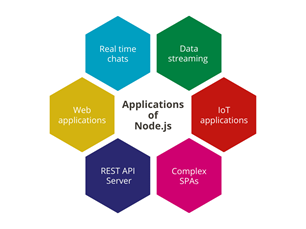
\includegraphics{media/NodeJs/NodeJsAnwendungen.png}
    \caption{Node.js Anwendungen \cite{AnwendungenFoto}}
\end{figure}

    \textbf{Chats in Echtzeit:}
    Die Node.js Architektur bietet eine Basis, um Echtzeit-Kommunikation zu verarbeiten. Durch die leichte Skalierbarkeit wird die Laufzeitumgebung oft bei der Entwicklung von Chatbots, zusätzlichen Chat-Funktionen wie "Multi-Person-Chats" und Push-Benachrichtigungen verwendet.

    \textbf{Internet of Things:}
    IoT-Anwendungen bestehen in den meisten Fällen aus mehreren Sensoren, die häufig, kleine Datenpakete senden. Aufgrund der immer mehr werdenden Anfragen bietet sich Node.js durch seine Eigenschaften umso mehr dafür an.

    \textbf{REST API-basierte Anwendungen:}
    Javascript wird nicht nur im Frontend, sondern auch im Backend von Webseiten eingesetzt. Mithilfe von Node.js besitzt ein Server somit die Möglichkeit, über REST APIs mit dem Frontend zu kommunizieren. Node.js bietet die Möglichkeit, Pakete zur Verfügung zu stellen und damit die Erstellung von Webanwendungen zu erleichtern. 

    \textbf{Daten-Streaming:}
    Bekannte Unternehmen wie "Netflix" und "Disney+" nutzen Node.js für Streamingzwecke, dies ist aufgrund der schnellen Laufzeitumgebung möglich. Wichtig zu erwähnen ist, dass eine native Streaming-API in Node.js schon vorweg implementiert ist.


\hfour{Hello World in Node.js}

Damit die neu entdeckte Programmiersprache erlernt wird, ist es oft so, dass man bei jeder neuen Programmiersprache ein netzwerkbasiertes "Hello World"-Programm schreibt. Dies sieht bei Node.js folgendermaßen aus:

\typescript{code/NodeJs/HelloWorld.ts}{HelloWorld in Node.js}

Im oben genannten Codebeispiel wird das http-Modul als erstes geladen. Danach wird die Methode "createServer" aufgerufen, um eine Anfrage anzunehmen und eine Antwort mit einem Statuscode zurückzugeben. Letztendlich wird auf einen Port gehört, der vordefiniert ist, ob Informationen an den Port gesendet werden.

Node.js wird den Entwicklern mit dem bereits eingebauten Modul namens "HTTP" bereitgestellt, welches die Datenübertragung über das "HyperText Transfer Protocol" (HTTP) ermöglicht. \cite{HelloWorld}

\pagebreak
\hfour{NPM}
\label{sec:npm}

"Der Node Package Manager (NPM) ist das Paket-System von Node.js". \cite{NPMIntro} Es ist das größte "Ecosystem" aller Open-Source Bibliotheken der Welt, mit über einer Millionen Pakete, weitere Pakete werden täglich releast. NPM ist kostenlos und hat eine sehr große Community, des öfteren Open Source Entwickler und begeisterte Programmierer. Die Firma, die hinter NPM steht, die sogenannte NPM INC., wurde 2014 gegründet und 2020 von GitHub aufgekauft.
NPM wird mit einem Kommandozeilenprogramm ausgeliefert. Die Möglichkeit besteht auch, auf der Webseite von NPM nach gewünschten Paketen zu suchen und diese mit einem einzigen Befehl zu installieren. Die Versionierung der Pakete und die Überprüfung von Abhängigkeiten kann eingerichtet werden. Node.js ist ein Dreh– und Angelpunkt für Entwickler*innen vor allem wegen dem "Package Support".
Die Sicherheit von Paketen ist bei NPM durch den bereits eingebauten Sicherheits-Scanner gegeben. \cite{NPM}\cite{NPM2}\cite{NPMIntro}


\begin{figure}[H]
    \centering
    
\includegraphics{media/NodeJs/NPM.png}
    \caption{NPM Logo \cite{NPMLOGO}}
\end{figure}

\begin{minipage}\textwidth
\hfive{Sicherheitslücken}
Wie jede Anwendung hat NPM anfänglich Probleme mit Sicherheitslücken gehabt, die zum Glück behoben werden konnten. Bei der ersten bekannten Sicherheitslücke, die nach der Übernahme von NPM durch GitHub im Jahr 2021 aufgetreten ist, war das Problem, dass neue Verisonen von beliebigen Paketen hochgeladen- und somit gesehen Pakete erschienen sind, die auch mögliche Schadsoftware beeinhalten könnten. Das genaue Datum des erstmaligen Auftretens des Fehlers ist unbekannt, jedoch wird vermutet, dass es mindestens seit September 2020 schon möglich gewesen wäre, diese Sicherheitslücke zu missbrauchen. \cite{NPMSecurity}
\end{minipage}


